\subsection{采样与量化的概念}

\begin{definition}[采样]
    把模拟信号变成数字信号时,每隔一个时间间隔
    在模拟信号波形上抽取一个幅度值,这称之为\bd{采样}。
    这是在某些\bd{离散}的时间点上提取\bd{连续}时间信号值的过程。

    采样的时间间隔称为\bd{采样周期} $T_s$,
    其倒数称为\bd{采样频率} $f_s = 1/T_s$。
    $\omega_s = 2\pi / T_s$ 称为\bd{采样角频率}。
\end{definition}

\begin{remark}
    在不发生混淆的情况下,$\omega_s$ 可简称为采样频率。
\end{remark}

\subsubsection{时域采样和幅度量化}

时域采样和幅度量化是数字信号处理的两个基本步骤,
如图 \ref{fig:sampling}、\ref{fig:quantize-1} 和 \ref{fig:quantize-2} 所示。
\begin{figure}[H]
    \centering
    \begin{subfigure}{0.30\textwidth}
        \centering
        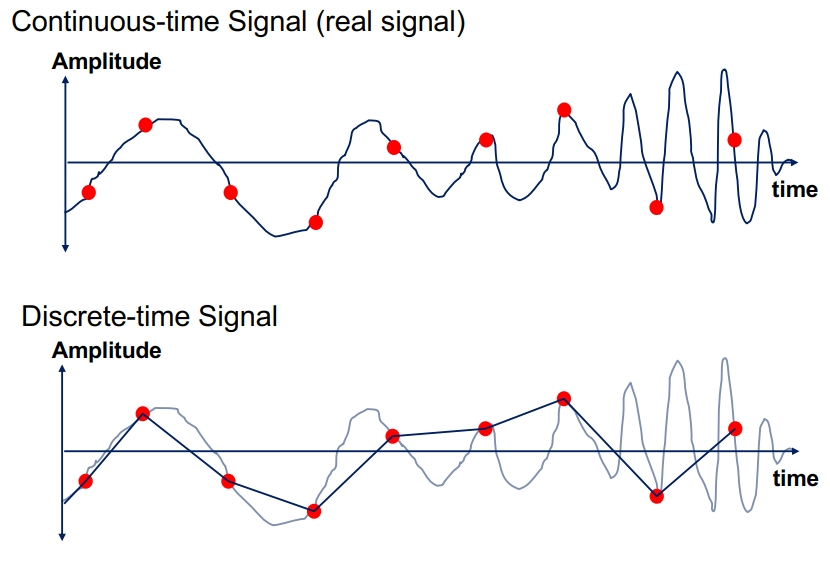
\includegraphics[width=\textwidth]{chap2/img/sampling.png}
        \caption{时域采样}
        \label{fig:sampling}
    \end{subfigure}
    \hfill
    \begin{subfigure}{0.30\textwidth}
        \centering
        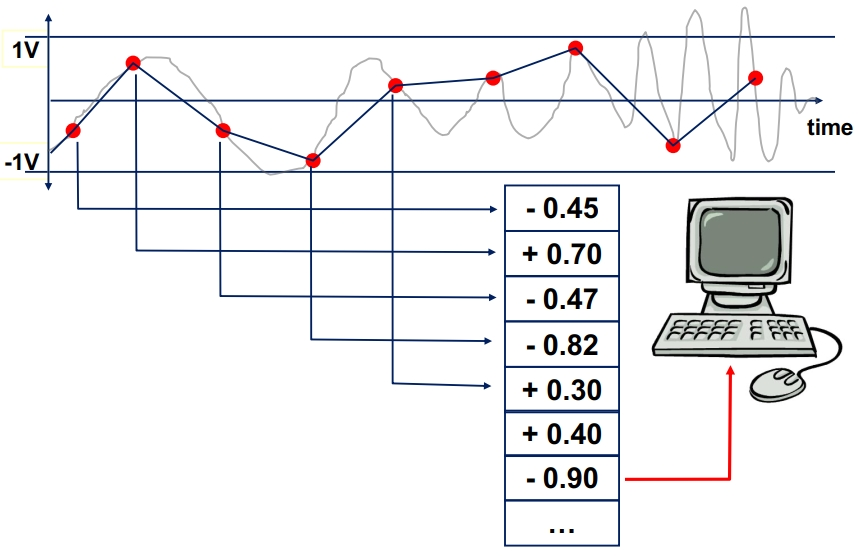
\includegraphics[width=\textwidth]{chap2/img/quantize-1.png}
        \caption{幅度量化(数据收集)}
        \label{fig:quantize-1}
    \end{subfigure}
    \hfill
    \begin{subfigure}{0.30\textwidth}
        \centering
        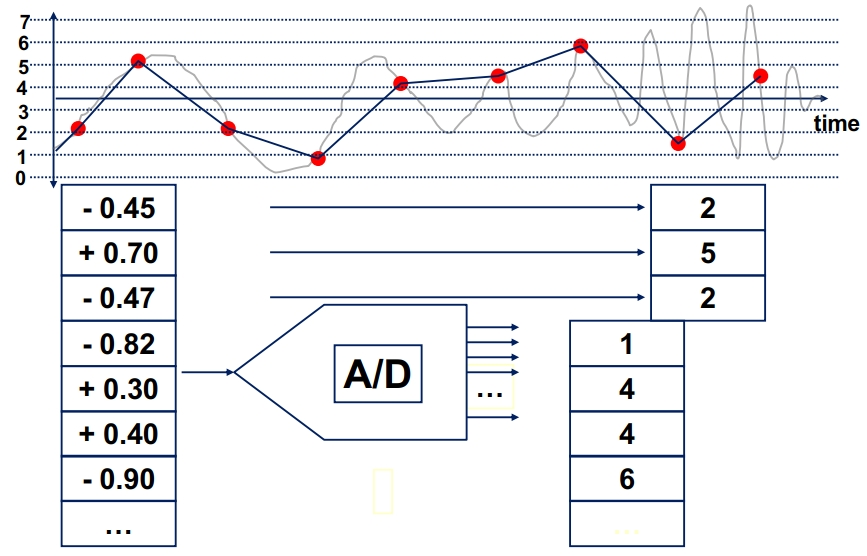
\includegraphics[width=\textwidth]{chap2/img/quantize-2.png}
        \caption{幅度量化(数据离散化)}
        \label{fig:quantize-2}
    \end{subfigure}
    \caption{时域采样和幅度量化}
\end{figure}

\subsubsection{采样的频率与分辨率}

采样的频率与分辨率会影响到信号的还原质量。
\begin{itemize}
    \item 采样频率升高,信号的还原质量会提高;但需要更大的存储空间(带宽)和成本。
    \item 采样分辨率升高,也能提高信号的还原质量;但需要更大的存储空间(精度)和成本。
\end{itemize}
如图 \ref{fig:sampling-frequency} 和 \ref{fig:sampling-resolution} 所示。
\begin{figure}[H]
    \centering
    \begin{subfigure}{0.45\textwidth}
        \centering
        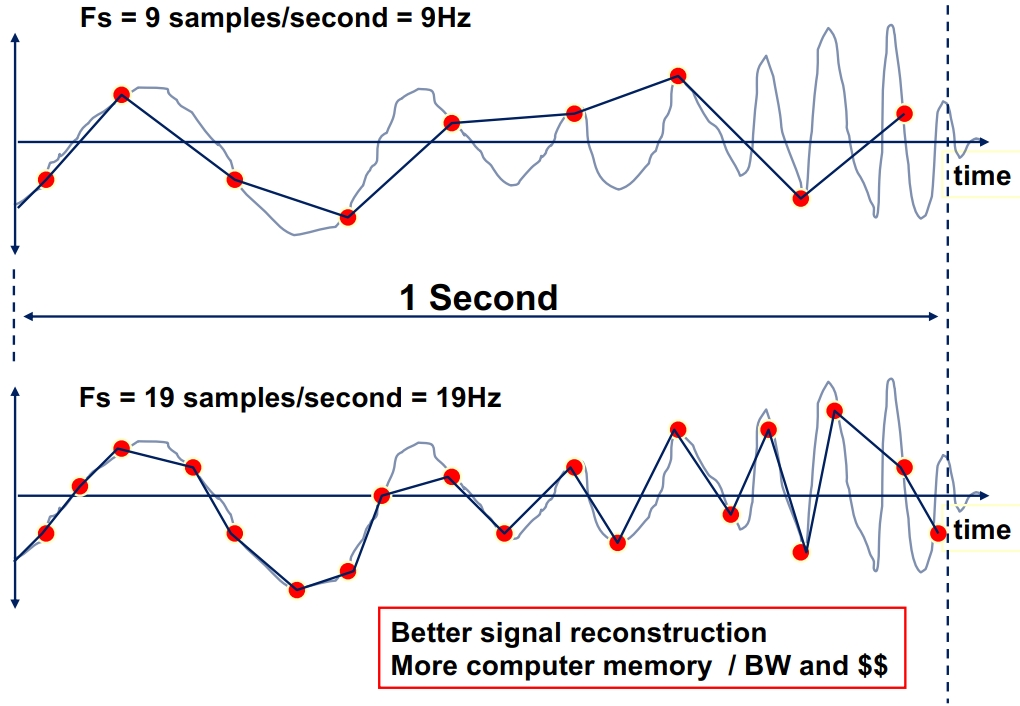
\includegraphics[width=\textwidth]{chap2/img/sampling-frequency.png}
        \caption{采样频率对信号还原的影响}
        \label{fig:sampling-frequency}
    \end{subfigure}
    \hfill
    \begin{subfigure}{0.45\textwidth}
        \centering
        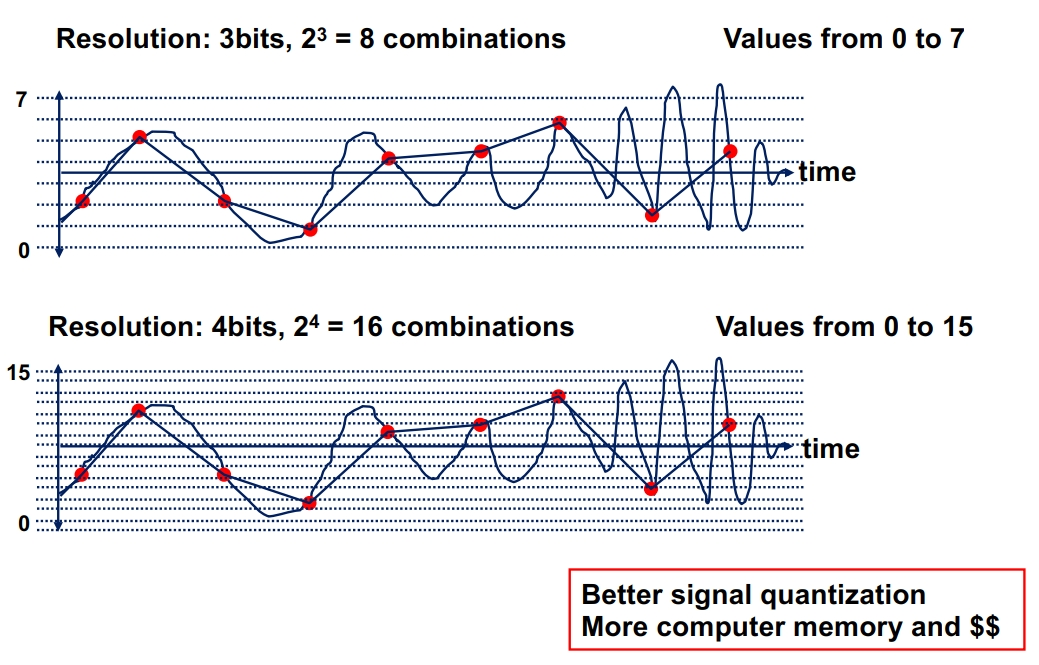
\includegraphics[width=\textwidth]{chap2/img/sampling-resolution.png}
        \caption{采样分辨率对信号还原的影响}
        \label{fig:sampling-resolution}
    \end{subfigure}
    \caption{采样频率与分辨率}
\end{figure}

\subsubsection{采样的应用}

在日常生活中,常可以看到用离散时间信号表示连续时间信号的例子。
如照片、屏幕的画面等等。在一定条件下,可以用离散时间信号代替连续时间信号。

\begin{example}[CCD 芯片的光显微图]
    CCD 芯片用 VLSI 技术制造。被分为许多微小区,当光成像在 CCD 芯片上时,
    就在这些空间离散的像素点上被采样,而生成了离散空间图像信号,
    如图 \ref{fig:ccd-chip} 所示。
    \begin{figure}[H]
        \centering
        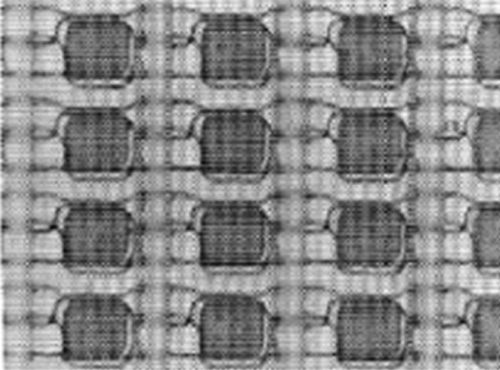
\includegraphics[width=0.45\textwidth]{chap2/img/ccd-chip.png}
        \caption{CCD 芯片的光显微图}
        \label{fig:ccd-chip}
    \end{figure}
\end{example}
